% Created by tikzDevice version 0.12.3.1 on 2022-03-28 12:20:56
% !TEX encoding = UTF-8 Unicode
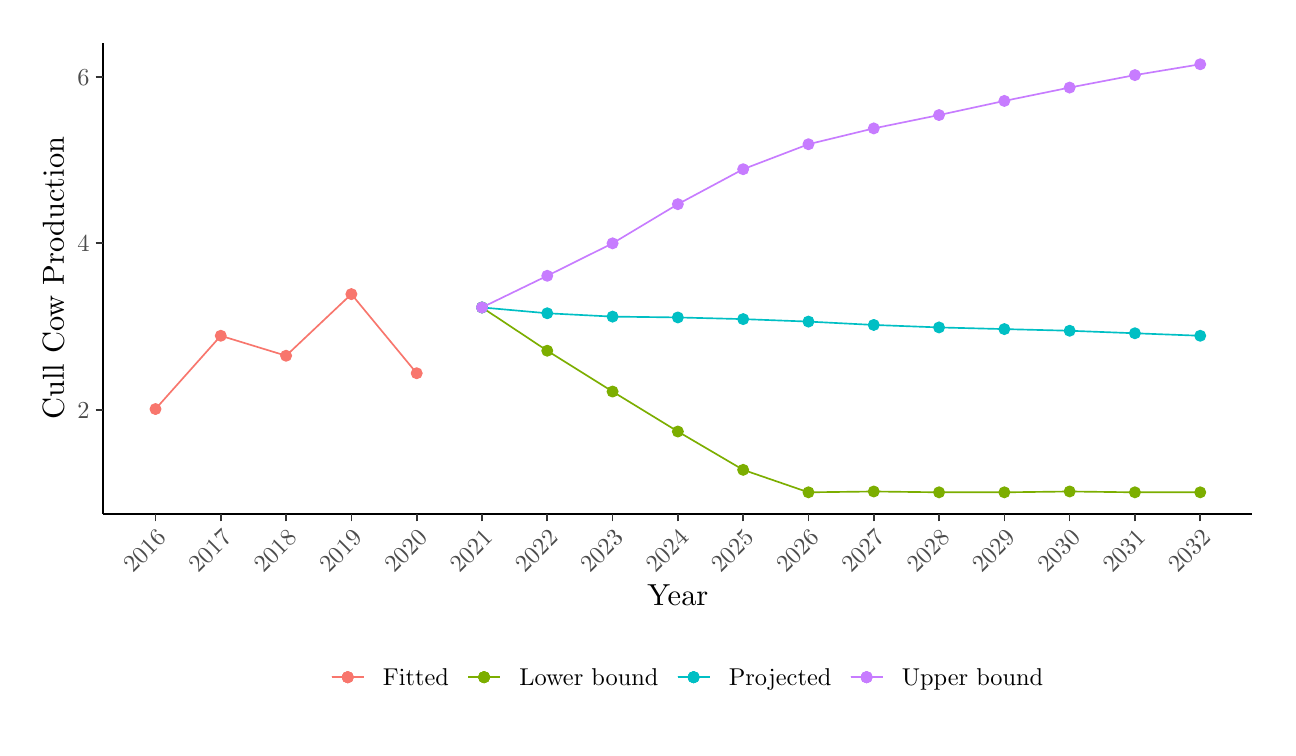
\begin{tikzpicture}[x=1pt,y=1pt]
\definecolor{fillColor}{RGB}{255,255,255}
\path[use as bounding box,fill=fillColor,fill opacity=0.00] (0,0) rectangle (448.07,252.94);
\begin{scope}
\path[clip] (  0.00,  0.00) rectangle (448.07,252.94);
\definecolor{drawColor}{RGB}{255,255,255}
\definecolor{fillColor}{RGB}{255,255,255}

\path[draw=drawColor,line width= 0.6pt,line join=round,line cap=round,fill=fillColor] (  0.00,  0.00) rectangle (448.07,252.94);
\end{scope}
\begin{scope}
\path[clip] ( 27.31, 77.31) rectangle (442.57,247.44);
\definecolor{fillColor}{RGB}{255,255,255}

\path[fill=fillColor] ( 27.31, 77.31) rectangle (442.57,247.44);
\definecolor{drawColor}{RGB}{248,118,109}

\path[draw=drawColor,line width= 0.6pt,line join=round] ( 46.19,115.13) --
	( 69.78,141.61) --
	( 93.38,134.39) --
	(116.97,156.66) --
	(140.57,128.07);
\definecolor{fillColor}{RGB}{248,118,109}

\path[draw=drawColor,line width= 0.4pt,line join=round,line cap=round,fill=fillColor] ( 46.19,115.13) circle (  1.96);

\path[draw=drawColor,line width= 0.4pt,line join=round,line cap=round,fill=fillColor] ( 69.78,141.61) circle (  1.96);

\path[draw=drawColor,line width= 0.4pt,line join=round,line cap=round,fill=fillColor] ( 93.38,134.39) circle (  1.96);

\path[draw=drawColor,line width= 0.4pt,line join=round,line cap=round,fill=fillColor] (116.97,156.66) circle (  1.96);

\path[draw=drawColor,line width= 0.4pt,line join=round,line cap=round,fill=fillColor] (140.57,128.07) circle (  1.96);
\definecolor{drawColor}{RGB}{124,174,0}

\path[draw=drawColor,line width= 0.6pt,line join=round] (164.16,151.84) --
	(187.75,136.20) --
	(211.35,121.45) --
	(234.94,107.01) --
	(258.54, 93.16) --
	(282.13, 85.04) --
	(305.73, 85.34) --
	(329.32, 85.04) --
	(352.92, 85.04) --
	(376.51, 85.34) --
	(400.10, 85.04) --
	(423.70, 85.04);
\definecolor{fillColor}{RGB}{124,174,0}

\path[draw=drawColor,line width= 0.4pt,line join=round,line cap=round,fill=fillColor] (164.16,151.84) circle (  1.96);

\path[draw=drawColor,line width= 0.4pt,line join=round,line cap=round,fill=fillColor] (187.75,136.20) circle (  1.96);

\path[draw=drawColor,line width= 0.4pt,line join=round,line cap=round,fill=fillColor] (211.35,121.45) circle (  1.96);

\path[draw=drawColor,line width= 0.4pt,line join=round,line cap=round,fill=fillColor] (234.94,107.01) circle (  1.96);

\path[draw=drawColor,line width= 0.4pt,line join=round,line cap=round,fill=fillColor] (258.54, 93.16) circle (  1.96);

\path[draw=drawColor,line width= 0.4pt,line join=round,line cap=round,fill=fillColor] (282.13, 85.04) circle (  1.96);

\path[draw=drawColor,line width= 0.4pt,line join=round,line cap=round,fill=fillColor] (305.73, 85.34) circle (  1.96);

\path[draw=drawColor,line width= 0.4pt,line join=round,line cap=round,fill=fillColor] (329.32, 85.04) circle (  1.96);

\path[draw=drawColor,line width= 0.4pt,line join=round,line cap=round,fill=fillColor] (352.92, 85.04) circle (  1.96);

\path[draw=drawColor,line width= 0.4pt,line join=round,line cap=round,fill=fillColor] (376.51, 85.34) circle (  1.96);

\path[draw=drawColor,line width= 0.4pt,line join=round,line cap=round,fill=fillColor] (400.10, 85.04) circle (  1.96);

\path[draw=drawColor,line width= 0.4pt,line join=round,line cap=round,fill=fillColor] (423.70, 85.04) circle (  1.96);
\definecolor{drawColor}{RGB}{0,191,196}

\path[draw=drawColor,line width= 0.6pt,line join=round] (164.16,151.84) --
	(187.75,149.74) --
	(211.35,148.53) --
	(234.94,148.23) --
	(258.54,147.63) --
	(282.13,146.73) --
	(305.73,145.52) --
	(329.32,144.62) --
	(352.92,144.02) --
	(376.51,143.42) --
	(400.10,142.51) --
	(423.70,141.61);
\definecolor{fillColor}{RGB}{0,191,196}

\path[draw=drawColor,line width= 0.4pt,line join=round,line cap=round,fill=fillColor] (164.16,151.84) circle (  1.96);

\path[draw=drawColor,line width= 0.4pt,line join=round,line cap=round,fill=fillColor] (187.75,149.74) circle (  1.96);

\path[draw=drawColor,line width= 0.4pt,line join=round,line cap=round,fill=fillColor] (211.35,148.53) circle (  1.96);

\path[draw=drawColor,line width= 0.4pt,line join=round,line cap=round,fill=fillColor] (234.94,148.23) circle (  1.96);

\path[draw=drawColor,line width= 0.4pt,line join=round,line cap=round,fill=fillColor] (258.54,147.63) circle (  1.96);

\path[draw=drawColor,line width= 0.4pt,line join=round,line cap=round,fill=fillColor] (282.13,146.73) circle (  1.96);

\path[draw=drawColor,line width= 0.4pt,line join=round,line cap=round,fill=fillColor] (305.73,145.52) circle (  1.96);

\path[draw=drawColor,line width= 0.4pt,line join=round,line cap=round,fill=fillColor] (329.32,144.62) circle (  1.96);

\path[draw=drawColor,line width= 0.4pt,line join=round,line cap=round,fill=fillColor] (352.92,144.02) circle (  1.96);

\path[draw=drawColor,line width= 0.4pt,line join=round,line cap=round,fill=fillColor] (376.51,143.42) circle (  1.96);

\path[draw=drawColor,line width= 0.4pt,line join=round,line cap=round,fill=fillColor] (400.10,142.51) circle (  1.96);

\path[draw=drawColor,line width= 0.4pt,line join=round,line cap=round,fill=fillColor] (423.70,141.61) circle (  1.96);
\definecolor{drawColor}{RGB}{199,124,255}

\path[draw=drawColor,line width= 0.6pt,line join=round] (164.16,151.84) --
	(187.75,163.28) --
	(211.35,175.01) --
	(234.94,189.16) --
	(258.54,201.80) --
	(282.13,210.82) --
	(305.73,216.54) --
	(329.32,221.36) --
	(352.92,226.47) --
	(376.51,231.29) --
	(400.10,235.80) --
	(423.70,239.71);
\definecolor{fillColor}{RGB}{199,124,255}

\path[draw=drawColor,line width= 0.4pt,line join=round,line cap=round,fill=fillColor] (164.16,151.84) circle (  1.96);

\path[draw=drawColor,line width= 0.4pt,line join=round,line cap=round,fill=fillColor] (187.75,163.28) circle (  1.96);

\path[draw=drawColor,line width= 0.4pt,line join=round,line cap=round,fill=fillColor] (211.35,175.01) circle (  1.96);

\path[draw=drawColor,line width= 0.4pt,line join=round,line cap=round,fill=fillColor] (234.94,189.16) circle (  1.96);

\path[draw=drawColor,line width= 0.4pt,line join=round,line cap=round,fill=fillColor] (258.54,201.80) circle (  1.96);

\path[draw=drawColor,line width= 0.4pt,line join=round,line cap=round,fill=fillColor] (282.13,210.82) circle (  1.96);

\path[draw=drawColor,line width= 0.4pt,line join=round,line cap=round,fill=fillColor] (305.73,216.54) circle (  1.96);

\path[draw=drawColor,line width= 0.4pt,line join=round,line cap=round,fill=fillColor] (329.32,221.36) circle (  1.96);

\path[draw=drawColor,line width= 0.4pt,line join=round,line cap=round,fill=fillColor] (352.92,226.47) circle (  1.96);

\path[draw=drawColor,line width= 0.4pt,line join=round,line cap=round,fill=fillColor] (376.51,231.29) circle (  1.96);

\path[draw=drawColor,line width= 0.4pt,line join=round,line cap=round,fill=fillColor] (400.10,235.80) circle (  1.96);

\path[draw=drawColor,line width= 0.4pt,line join=round,line cap=round,fill=fillColor] (423.70,239.71) circle (  1.96);
\end{scope}
\begin{scope}
\path[clip] (  0.00,  0.00) rectangle (448.07,252.94);
\definecolor{drawColor}{RGB}{0,0,0}

\path[draw=drawColor,line width= 0.6pt,line join=round] ( 27.31, 77.31) --
	( 27.31,247.44);
\end{scope}
\begin{scope}
\path[clip] (  0.00,  0.00) rectangle (448.07,252.94);
\definecolor{drawColor}{gray}{0.30}

\node[text=drawColor,anchor=base east,inner sep=0pt, outer sep=0pt, scale=  0.88] at ( 22.36,111.80) {2};

\node[text=drawColor,anchor=base east,inner sep=0pt, outer sep=0pt, scale=  0.88] at ( 22.36,171.98) {4};

\node[text=drawColor,anchor=base east,inner sep=0pt, outer sep=0pt, scale=  0.88] at ( 22.36,232.17) {6};
\end{scope}
\begin{scope}
\path[clip] (  0.00,  0.00) rectangle (448.07,252.94);
\definecolor{drawColor}{gray}{0.20}

\path[draw=drawColor,line width= 0.6pt,line join=round] ( 24.56,114.83) --
	( 27.31,114.83);

\path[draw=drawColor,line width= 0.6pt,line join=round] ( 24.56,175.01) --
	( 27.31,175.01);

\path[draw=drawColor,line width= 0.6pt,line join=round] ( 24.56,235.20) --
	( 27.31,235.20);
\end{scope}
\begin{scope}
\path[clip] (  0.00,  0.00) rectangle (448.07,252.94);
\definecolor{drawColor}{RGB}{0,0,0}

\path[draw=drawColor,line width= 0.6pt,line join=round] ( 27.31, 77.31) --
	(442.57, 77.31);
\end{scope}
\begin{scope}
\path[clip] (  0.00,  0.00) rectangle (448.07,252.94);
\definecolor{drawColor}{gray}{0.20}

\path[draw=drawColor,line width= 0.6pt,line join=round] ( 46.19, 74.56) --
	( 46.19, 77.31);

\path[draw=drawColor,line width= 0.6pt,line join=round] ( 69.78, 74.56) --
	( 69.78, 77.31);

\path[draw=drawColor,line width= 0.6pt,line join=round] ( 93.38, 74.56) --
	( 93.38, 77.31);

\path[draw=drawColor,line width= 0.6pt,line join=round] (116.97, 74.56) --
	(116.97, 77.31);

\path[draw=drawColor,line width= 0.6pt,line join=round] (140.57, 74.56) --
	(140.57, 77.31);

\path[draw=drawColor,line width= 0.6pt,line join=round] (164.16, 74.56) --
	(164.16, 77.31);

\path[draw=drawColor,line width= 0.6pt,line join=round] (187.75, 74.56) --
	(187.75, 77.31);

\path[draw=drawColor,line width= 0.6pt,line join=round] (211.35, 74.56) --
	(211.35, 77.31);

\path[draw=drawColor,line width= 0.6pt,line join=round] (234.94, 74.56) --
	(234.94, 77.31);

\path[draw=drawColor,line width= 0.6pt,line join=round] (258.54, 74.56) --
	(258.54, 77.31);

\path[draw=drawColor,line width= 0.6pt,line join=round] (282.13, 74.56) --
	(282.13, 77.31);

\path[draw=drawColor,line width= 0.6pt,line join=round] (305.73, 74.56) --
	(305.73, 77.31);

\path[draw=drawColor,line width= 0.6pt,line join=round] (329.32, 74.56) --
	(329.32, 77.31);

\path[draw=drawColor,line width= 0.6pt,line join=round] (352.92, 74.56) --
	(352.92, 77.31);

\path[draw=drawColor,line width= 0.6pt,line join=round] (376.51, 74.56) --
	(376.51, 77.31);

\path[draw=drawColor,line width= 0.6pt,line join=round] (400.10, 74.56) --
	(400.10, 77.31);

\path[draw=drawColor,line width= 0.6pt,line join=round] (423.70, 74.56) --
	(423.70, 77.31);
\end{scope}
\begin{scope}
\path[clip] (  0.00,  0.00) rectangle (448.07,252.94);
\definecolor{drawColor}{gray}{0.30}

\node[text=drawColor,rotate= 45.00,anchor=base east,inner sep=0pt, outer sep=0pt, scale=  0.88] at ( 50.47, 68.07) {2016};

\node[text=drawColor,rotate= 45.00,anchor=base east,inner sep=0pt, outer sep=0pt, scale=  0.88] at ( 74.07, 68.07) {2017};

\node[text=drawColor,rotate= 45.00,anchor=base east,inner sep=0pt, outer sep=0pt, scale=  0.88] at ( 97.66, 68.07) {2018};

\node[text=drawColor,rotate= 45.00,anchor=base east,inner sep=0pt, outer sep=0pt, scale=  0.88] at (121.26, 68.07) {2019};

\node[text=drawColor,rotate= 45.00,anchor=base east,inner sep=0pt, outer sep=0pt, scale=  0.88] at (144.85, 68.07) {2020};

\node[text=drawColor,rotate= 45.00,anchor=base east,inner sep=0pt, outer sep=0pt, scale=  0.88] at (168.45, 68.07) {2021};

\node[text=drawColor,rotate= 45.00,anchor=base east,inner sep=0pt, outer sep=0pt, scale=  0.88] at (192.04, 68.07) {2022};

\node[text=drawColor,rotate= 45.00,anchor=base east,inner sep=0pt, outer sep=0pt, scale=  0.88] at (215.63, 68.07) {2023};

\node[text=drawColor,rotate= 45.00,anchor=base east,inner sep=0pt, outer sep=0pt, scale=  0.88] at (239.23, 68.07) {2024};

\node[text=drawColor,rotate= 45.00,anchor=base east,inner sep=0pt, outer sep=0pt, scale=  0.88] at (262.82, 68.07) {2025};

\node[text=drawColor,rotate= 45.00,anchor=base east,inner sep=0pt, outer sep=0pt, scale=  0.88] at (286.42, 68.07) {2026};

\node[text=drawColor,rotate= 45.00,anchor=base east,inner sep=0pt, outer sep=0pt, scale=  0.88] at (310.01, 68.07) {2027};

\node[text=drawColor,rotate= 45.00,anchor=base east,inner sep=0pt, outer sep=0pt, scale=  0.88] at (333.61, 68.07) {2028};

\node[text=drawColor,rotate= 45.00,anchor=base east,inner sep=0pt, outer sep=0pt, scale=  0.88] at (357.20, 68.07) {2029};

\node[text=drawColor,rotate= 45.00,anchor=base east,inner sep=0pt, outer sep=0pt, scale=  0.88] at (380.80, 68.07) {2030};

\node[text=drawColor,rotate= 45.00,anchor=base east,inner sep=0pt, outer sep=0pt, scale=  0.88] at (404.39, 68.07) {2031};

\node[text=drawColor,rotate= 45.00,anchor=base east,inner sep=0pt, outer sep=0pt, scale=  0.88] at (427.98, 68.07) {2032};
\end{scope}
\begin{scope}
\path[clip] (  0.00,  0.00) rectangle (448.07,252.94);
\definecolor{drawColor}{RGB}{0,0,0}

\node[text=drawColor,anchor=base,inner sep=0pt, outer sep=0pt, scale=  1.10] at (234.94, 44.09) {Year};
\end{scope}
\begin{scope}
\path[clip] (  0.00,  0.00) rectangle (448.07,252.94);
\definecolor{drawColor}{RGB}{0,0,0}

\node[text=drawColor,rotate= 90.00,anchor=base,inner sep=0pt, outer sep=0pt, scale=  1.10] at ( 13.08,162.38) {Cull Cow Production};
\end{scope}
\begin{scope}
\path[clip] (  0.00,  0.00) rectangle (448.07,252.94);
\definecolor{fillColor}{RGB}{255,255,255}

\path[fill=fillColor] ( 97.42,  5.50) rectangle (372.46, 30.95);
\end{scope}
\begin{scope}
\path[clip] (  0.00,  0.00) rectangle (448.07,252.94);
\definecolor{drawColor}{RGB}{248,118,109}

\path[draw=drawColor,line width= 0.6pt,line join=round] (109.87, 18.23) -- (121.43, 18.23);
\end{scope}
\begin{scope}
\path[clip] (  0.00,  0.00) rectangle (448.07,252.94);
\definecolor{drawColor}{RGB}{248,118,109}
\definecolor{fillColor}{RGB}{248,118,109}

\path[draw=drawColor,line width= 0.4pt,line join=round,line cap=round,fill=fillColor] (115.65, 18.23) circle (  1.96);
\end{scope}
\begin{scope}
\path[clip] (  0.00,  0.00) rectangle (448.07,252.94);
\definecolor{drawColor}{RGB}{248,118,109}

\path[draw=drawColor,line width= 0.6pt,line join=round] (109.87, 18.23) -- (121.43, 18.23);
\end{scope}
\begin{scope}
\path[clip] (  0.00,  0.00) rectangle (448.07,252.94);
\definecolor{drawColor}{RGB}{248,118,109}
\definecolor{fillColor}{RGB}{248,118,109}

\path[draw=drawColor,line width= 0.4pt,line join=round,line cap=round,fill=fillColor] (115.65, 18.23) circle (  1.96);
\end{scope}
\begin{scope}
\path[clip] (  0.00,  0.00) rectangle (448.07,252.94);
\definecolor{drawColor}{RGB}{248,118,109}

\path[draw=drawColor,line width= 0.6pt,line join=round] (109.87, 18.23) -- (121.43, 18.23);
\end{scope}
\begin{scope}
\path[clip] (  0.00,  0.00) rectangle (448.07,252.94);
\definecolor{drawColor}{RGB}{248,118,109}
\definecolor{fillColor}{RGB}{248,118,109}

\path[draw=drawColor,line width= 0.4pt,line join=round,line cap=round,fill=fillColor] (115.65, 18.23) circle (  1.96);
\end{scope}
\begin{scope}
\path[clip] (  0.00,  0.00) rectangle (448.07,252.94);
\definecolor{drawColor}{RGB}{248,118,109}

\path[draw=drawColor,line width= 0.6pt,line join=round] (109.87, 18.23) -- (121.43, 18.23);
\end{scope}
\begin{scope}
\path[clip] (  0.00,  0.00) rectangle (448.07,252.94);
\definecolor{drawColor}{RGB}{248,118,109}
\definecolor{fillColor}{RGB}{248,118,109}

\path[draw=drawColor,line width= 0.4pt,line join=round,line cap=round,fill=fillColor] (115.65, 18.23) circle (  1.96);
\end{scope}
\begin{scope}
\path[clip] (  0.00,  0.00) rectangle (448.07,252.94);
\definecolor{drawColor}{RGB}{124,174,0}

\path[draw=drawColor,line width= 0.6pt,line join=round] (159.15, 18.23) -- (170.71, 18.23);
\end{scope}
\begin{scope}
\path[clip] (  0.00,  0.00) rectangle (448.07,252.94);
\definecolor{drawColor}{RGB}{124,174,0}
\definecolor{fillColor}{RGB}{124,174,0}

\path[draw=drawColor,line width= 0.4pt,line join=round,line cap=round,fill=fillColor] (164.93, 18.23) circle (  1.96);
\end{scope}
\begin{scope}
\path[clip] (  0.00,  0.00) rectangle (448.07,252.94);
\definecolor{drawColor}{RGB}{124,174,0}

\path[draw=drawColor,line width= 0.6pt,line join=round] (159.15, 18.23) -- (170.71, 18.23);
\end{scope}
\begin{scope}
\path[clip] (  0.00,  0.00) rectangle (448.07,252.94);
\definecolor{drawColor}{RGB}{124,174,0}
\definecolor{fillColor}{RGB}{124,174,0}

\path[draw=drawColor,line width= 0.4pt,line join=round,line cap=round,fill=fillColor] (164.93, 18.23) circle (  1.96);
\end{scope}
\begin{scope}
\path[clip] (  0.00,  0.00) rectangle (448.07,252.94);
\definecolor{drawColor}{RGB}{124,174,0}

\path[draw=drawColor,line width= 0.6pt,line join=round] (159.15, 18.23) -- (170.71, 18.23);
\end{scope}
\begin{scope}
\path[clip] (  0.00,  0.00) rectangle (448.07,252.94);
\definecolor{drawColor}{RGB}{124,174,0}
\definecolor{fillColor}{RGB}{124,174,0}

\path[draw=drawColor,line width= 0.4pt,line join=round,line cap=round,fill=fillColor] (164.93, 18.23) circle (  1.96);
\end{scope}
\begin{scope}
\path[clip] (  0.00,  0.00) rectangle (448.07,252.94);
\definecolor{drawColor}{RGB}{124,174,0}

\path[draw=drawColor,line width= 0.6pt,line join=round] (159.15, 18.23) -- (170.71, 18.23);
\end{scope}
\begin{scope}
\path[clip] (  0.00,  0.00) rectangle (448.07,252.94);
\definecolor{drawColor}{RGB}{124,174,0}
\definecolor{fillColor}{RGB}{124,174,0}

\path[draw=drawColor,line width= 0.4pt,line join=round,line cap=round,fill=fillColor] (164.93, 18.23) circle (  1.96);
\end{scope}
\begin{scope}
\path[clip] (  0.00,  0.00) rectangle (448.07,252.94);
\definecolor{drawColor}{RGB}{0,191,196}

\path[draw=drawColor,line width= 0.6pt,line join=round] (234.85, 18.23) -- (246.41, 18.23);
\end{scope}
\begin{scope}
\path[clip] (  0.00,  0.00) rectangle (448.07,252.94);
\definecolor{drawColor}{RGB}{0,191,196}
\definecolor{fillColor}{RGB}{0,191,196}

\path[draw=drawColor,line width= 0.4pt,line join=round,line cap=round,fill=fillColor] (240.63, 18.23) circle (  1.96);
\end{scope}
\begin{scope}
\path[clip] (  0.00,  0.00) rectangle (448.07,252.94);
\definecolor{drawColor}{RGB}{0,191,196}

\path[draw=drawColor,line width= 0.6pt,line join=round] (234.85, 18.23) -- (246.41, 18.23);
\end{scope}
\begin{scope}
\path[clip] (  0.00,  0.00) rectangle (448.07,252.94);
\definecolor{drawColor}{RGB}{0,191,196}
\definecolor{fillColor}{RGB}{0,191,196}

\path[draw=drawColor,line width= 0.4pt,line join=round,line cap=round,fill=fillColor] (240.63, 18.23) circle (  1.96);
\end{scope}
\begin{scope}
\path[clip] (  0.00,  0.00) rectangle (448.07,252.94);
\definecolor{drawColor}{RGB}{0,191,196}

\path[draw=drawColor,line width= 0.6pt,line join=round] (234.85, 18.23) -- (246.41, 18.23);
\end{scope}
\begin{scope}
\path[clip] (  0.00,  0.00) rectangle (448.07,252.94);
\definecolor{drawColor}{RGB}{0,191,196}
\definecolor{fillColor}{RGB}{0,191,196}

\path[draw=drawColor,line width= 0.4pt,line join=round,line cap=round,fill=fillColor] (240.63, 18.23) circle (  1.96);
\end{scope}
\begin{scope}
\path[clip] (  0.00,  0.00) rectangle (448.07,252.94);
\definecolor{drawColor}{RGB}{0,191,196}

\path[draw=drawColor,line width= 0.6pt,line join=round] (234.85, 18.23) -- (246.41, 18.23);
\end{scope}
\begin{scope}
\path[clip] (  0.00,  0.00) rectangle (448.07,252.94);
\definecolor{drawColor}{RGB}{0,191,196}
\definecolor{fillColor}{RGB}{0,191,196}

\path[draw=drawColor,line width= 0.4pt,line join=round,line cap=round,fill=fillColor] (240.63, 18.23) circle (  1.96);
\end{scope}
\begin{scope}
\path[clip] (  0.00,  0.00) rectangle (448.07,252.94);
\definecolor{drawColor}{RGB}{199,124,255}

\path[draw=drawColor,line width= 0.6pt,line join=round] (297.35, 18.23) -- (308.92, 18.23);
\end{scope}
\begin{scope}
\path[clip] (  0.00,  0.00) rectangle (448.07,252.94);
\definecolor{drawColor}{RGB}{199,124,255}
\definecolor{fillColor}{RGB}{199,124,255}

\path[draw=drawColor,line width= 0.4pt,line join=round,line cap=round,fill=fillColor] (303.14, 18.23) circle (  1.96);
\end{scope}
\begin{scope}
\path[clip] (  0.00,  0.00) rectangle (448.07,252.94);
\definecolor{drawColor}{RGB}{199,124,255}

\path[draw=drawColor,line width= 0.6pt,line join=round] (297.35, 18.23) -- (308.92, 18.23);
\end{scope}
\begin{scope}
\path[clip] (  0.00,  0.00) rectangle (448.07,252.94);
\definecolor{drawColor}{RGB}{199,124,255}
\definecolor{fillColor}{RGB}{199,124,255}

\path[draw=drawColor,line width= 0.4pt,line join=round,line cap=round,fill=fillColor] (303.14, 18.23) circle (  1.96);
\end{scope}
\begin{scope}
\path[clip] (  0.00,  0.00) rectangle (448.07,252.94);
\definecolor{drawColor}{RGB}{199,124,255}

\path[draw=drawColor,line width= 0.6pt,line join=round] (297.35, 18.23) -- (308.92, 18.23);
\end{scope}
\begin{scope}
\path[clip] (  0.00,  0.00) rectangle (448.07,252.94);
\definecolor{drawColor}{RGB}{199,124,255}
\definecolor{fillColor}{RGB}{199,124,255}

\path[draw=drawColor,line width= 0.4pt,line join=round,line cap=round,fill=fillColor] (303.14, 18.23) circle (  1.96);
\end{scope}
\begin{scope}
\path[clip] (  0.00,  0.00) rectangle (448.07,252.94);
\definecolor{drawColor}{RGB}{199,124,255}

\path[draw=drawColor,line width= 0.6pt,line join=round] (297.35, 18.23) -- (308.92, 18.23);
\end{scope}
\begin{scope}
\path[clip] (  0.00,  0.00) rectangle (448.07,252.94);
\definecolor{drawColor}{RGB}{199,124,255}
\definecolor{fillColor}{RGB}{199,124,255}

\path[draw=drawColor,line width= 0.4pt,line join=round,line cap=round,fill=fillColor] (303.14, 18.23) circle (  1.96);
\end{scope}
\begin{scope}
\path[clip] (  0.00,  0.00) rectangle (448.07,252.94);
\definecolor{drawColor}{RGB}{0,0,0}

\node[text=drawColor,anchor=base west,inner sep=0pt, outer sep=0pt, scale=  0.88] at (128.38, 15.20) {Fitted};
\end{scope}
\begin{scope}
\path[clip] (  0.00,  0.00) rectangle (448.07,252.94);
\definecolor{drawColor}{RGB}{0,0,0}

\node[text=drawColor,anchor=base west,inner sep=0pt, outer sep=0pt, scale=  0.88] at (177.66, 15.20) {Lower bound};
\end{scope}
\begin{scope}
\path[clip] (  0.00,  0.00) rectangle (448.07,252.94);
\definecolor{drawColor}{RGB}{0,0,0}

\node[text=drawColor,anchor=base west,inner sep=0pt, outer sep=0pt, scale=  0.88] at (253.36, 15.20) {Projected};
\end{scope}
\begin{scope}
\path[clip] (  0.00,  0.00) rectangle (448.07,252.94);
\definecolor{drawColor}{RGB}{0,0,0}

\node[text=drawColor,anchor=base west,inner sep=0pt, outer sep=0pt, scale=  0.88] at (315.86, 15.20) {Upper bound};
\end{scope}
\end{tikzpicture}
